


\documentclass[20pt,usenames,dvipsnames]{beamer}

\usepackage[ngerman,english]{babel}
\usepackage{tikz}
 \usetikzlibrary{arrows,topaths}
\usepackage[normalem]{ulem}
\geometry{paperwidth=10in, paperheight=7.5in}
\usepackage{animate}

\usepackage[utf8]{inputenc}

\usepackage[mpidr]{./mpidr/beamerthemeMPIDR}
%\usefonttheme{serif}
%\newcolumntype{C}[1]{>{\centering\let\newline\\\arraybackslash\hspace{0pt}}m{#1}}
%\newcommand*{\QEDA}{\hfill\ensuremath{\blacksquare}}
%% Declaring title and author
%	the institute's logo
%\renewcommand{\mylogo}{\includegraphics[width=4.7in]{mpidr_logo_colour_en}}
\usepackage{color}
\definecolor{mygray}{rgb}{0.8,0.8,0.8}
\definecolor{yellow}{rgb}{1,1,0}
\usepackage[most]{tcolorbox}
\usepackage{xcolor,colortbl}
\usepackage{booktabs}
\usepackage{tabularx}
\defbeamertemplate{description item}{align left}{\insertdescriptionitem\hfill}
%%	should be the very last package to be loaded
\usepackage{hyperref}

%%%%%%%%%%%%%%%%%%%%%%%%%%%%%%%%%%
%%	Beginning of the document		%%
%%%%%%%%%%%%%%%%%%%%%%%%%%%%%%%%%%
\begin{document}

%%	titlepage - fixed frame:
%%	========================

% \begin{frame}
% 	\titlepage
% \end{frame}
\begin{frame}[plain]
	%\titlepage
	\vspace{-3cm}
 \centerline{\includegraphics[scale=.165]{beamerstrip3.png}}
	\huge
	\vspace{1em}
	
	Healthy lives: Delayed onset, improved recovery, or mortality
change?\\
	\vspace{1em}
	\large 
	Tim Riffe, Neil Mehta, Daniel Schneider, Mikko Myrskyl\"a 
\end{frame}
%-------------------
\begin{frame}[plain]
\Large
\begin{block}{Objective}
How much of the change in life expectancy at age 50 $e(50)$ is due to changes in mortality versus changes in disability transitions?
\end{block}
\end{frame}
%-------------------
\begin{frame}[plain]
\Large
\begin{block}{Data \& Methods}
\begin{itemize}[<+->]
\item HRS RAND version P. 
\item Transition probabilities: mlogit with age splines (3 knots).
\item Controls for race/eth (4) and education (3). 
\item 3-state Markov matrix models centered on years 1996, 2006, and 2014. 
\item Trend decomposition using Horiuchi et. al. (2007) method.
\end{itemize}
\end{block}
\end{frame}

\begin{frame}[plain]
\Large
\begin{center}
%\begin{tikzpicture}[->,auto,node distance=5cm,
%  thick,main node/.style={draw}]
  \begin{tikzpicture}[>=stealth',semithick,
  auto, node distance = 3cm,main node/.style={draw}]

  \node[main node] at (0,0) (1) {Disability free};
  \node[main node] at (5,-7) (3)  {Dead};
  \node[main node] at (10,0) (2)  {Disabled};

  \path[every node/.style={font=\sffamily\small}]
    (1) edge [bend right] node [left] {die healthy} (3)
    (1) edge [bend right] node [below] {disablement} (2)
    (1) edge [loop left] node {} (1)
    (2) edge [bend right] node [above] {recovery} (1)
    (2) edge [loop right] node {} (2)
    (2) edge [bend left] node {die disabled} (3)
    (3) edge [loop below] node {} (3);
    
\end{tikzpicture}
\end{center}
\end{frame}

\begin{frame}[plain]
\vspace{-1em}
\begin{center}
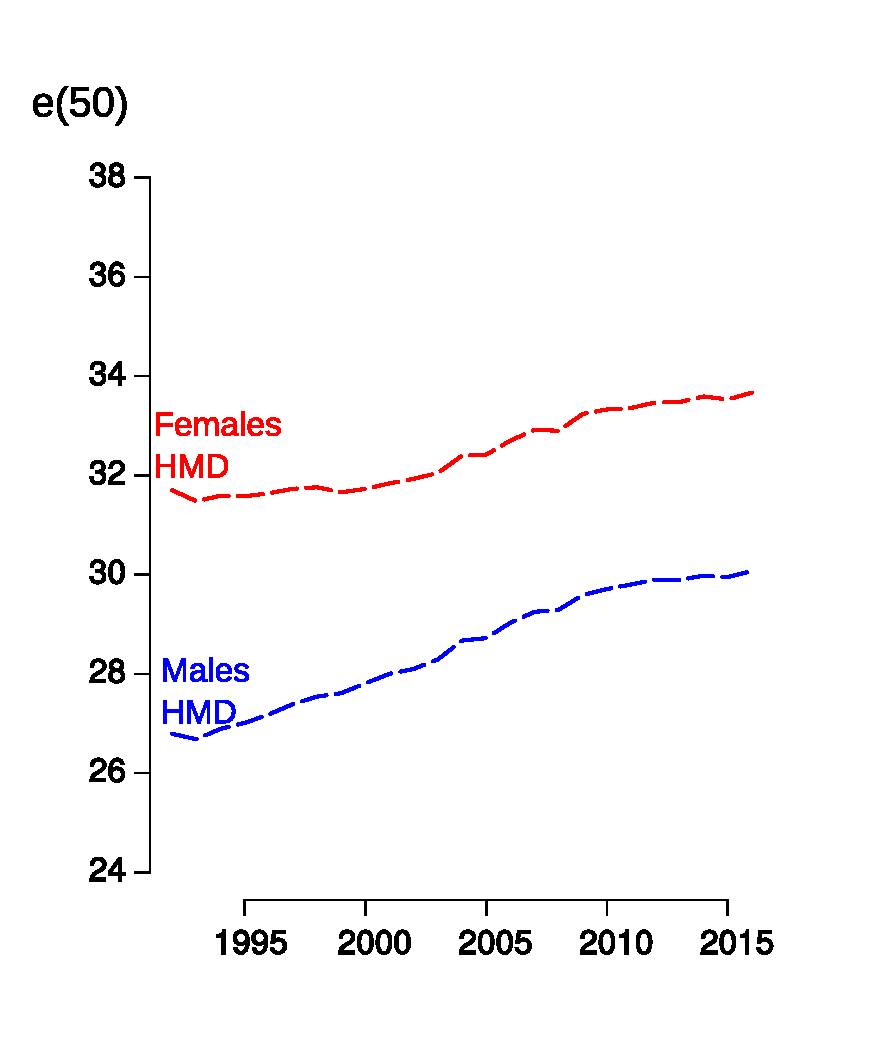
\includegraphics[height=20cm, keepaspectratio]{Figures/e50_0.pdf}
\end{center}
\end{frame}
\begin{frame}[plain]
\vspace{-1em}
\begin{center}
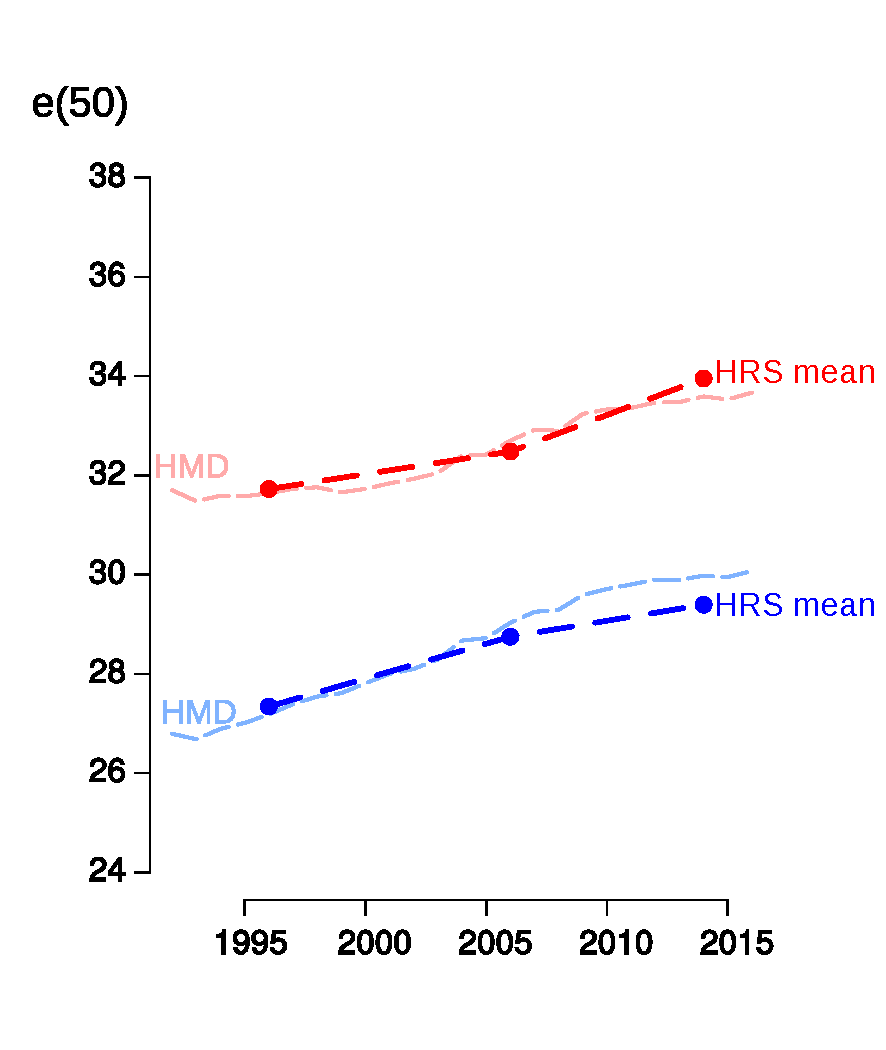
\includegraphics[height=20cm, keepaspectratio]{Figures/e50_1.pdf}
\end{center}
\end{frame}

%\begin{overlayarea}{\textwidth}{.8\textheight}
%\begin{center}
%\only<1>{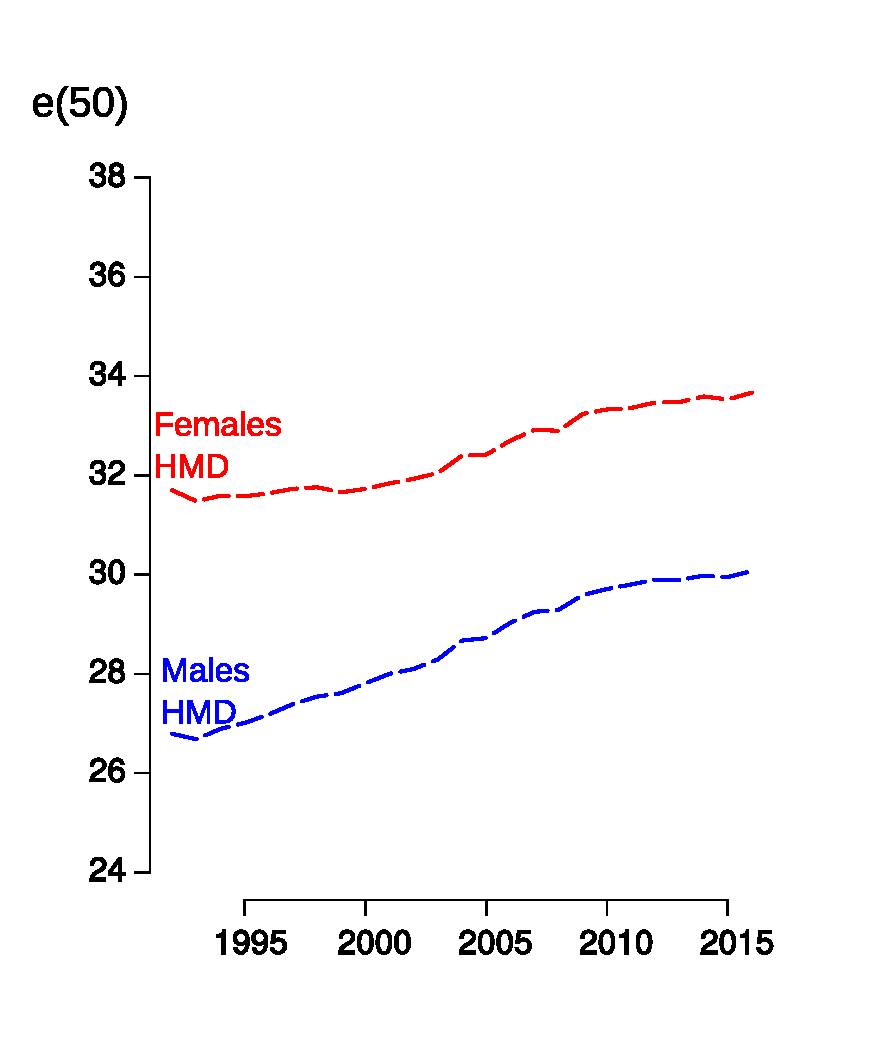
\includegraphics[height=\textheight, keepaspectratio]{Figures/e50_0.pdf}}
%\only<2>{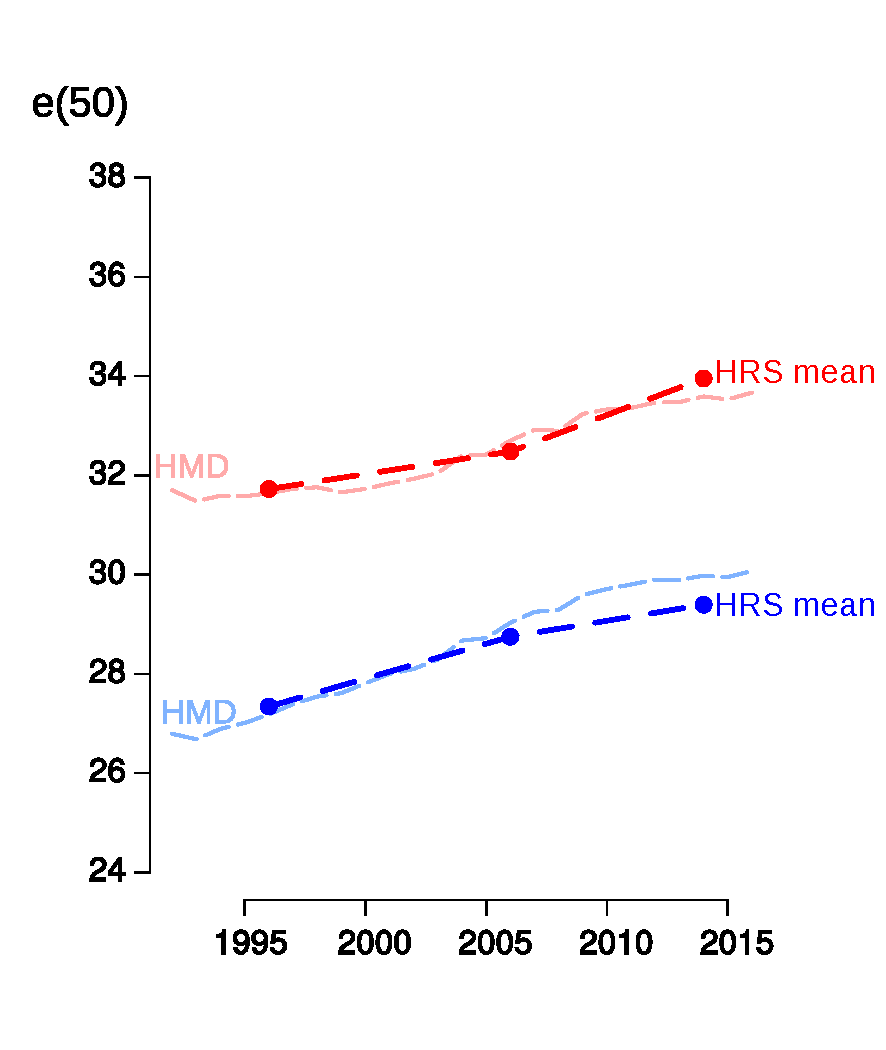
\includegraphics[height=\textheight, keepaspectratio]{Figures/e50_1.pdf}}
%\only<3>{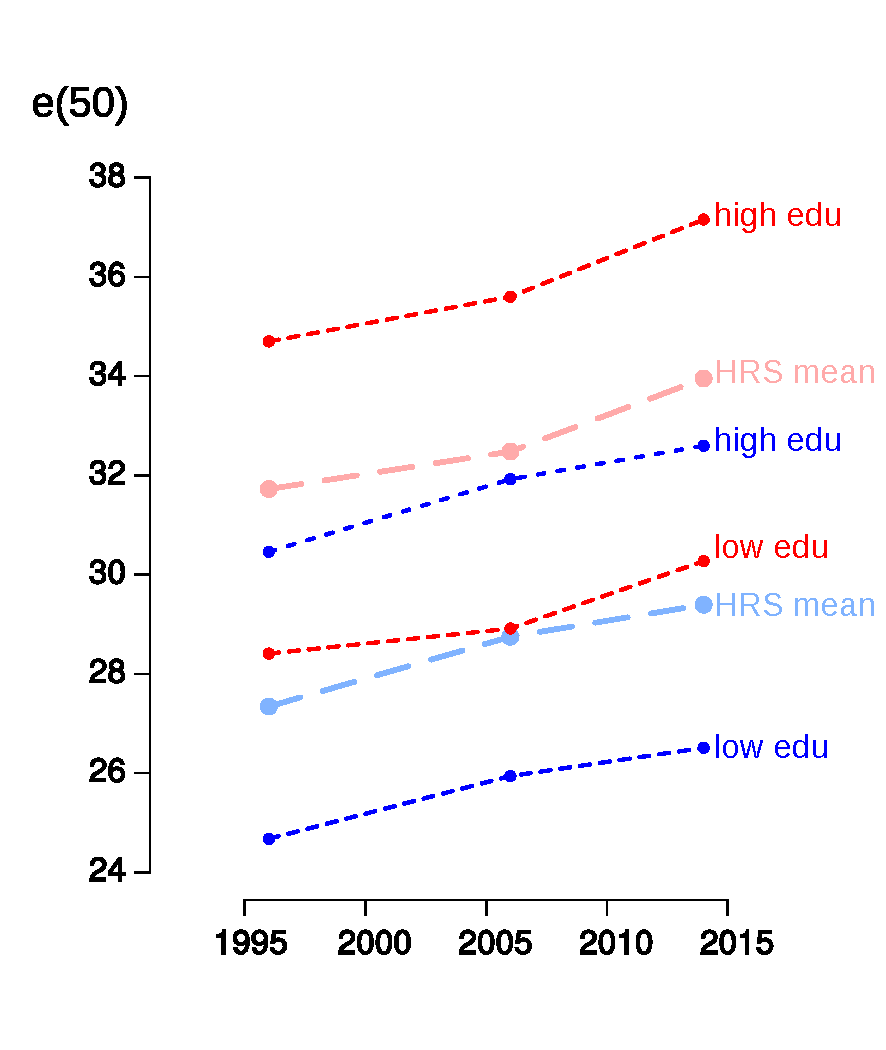
\includegraphics[height=\textheight, keepaspectratio]{Figures/e50_2.pdf}}
%\only<4>{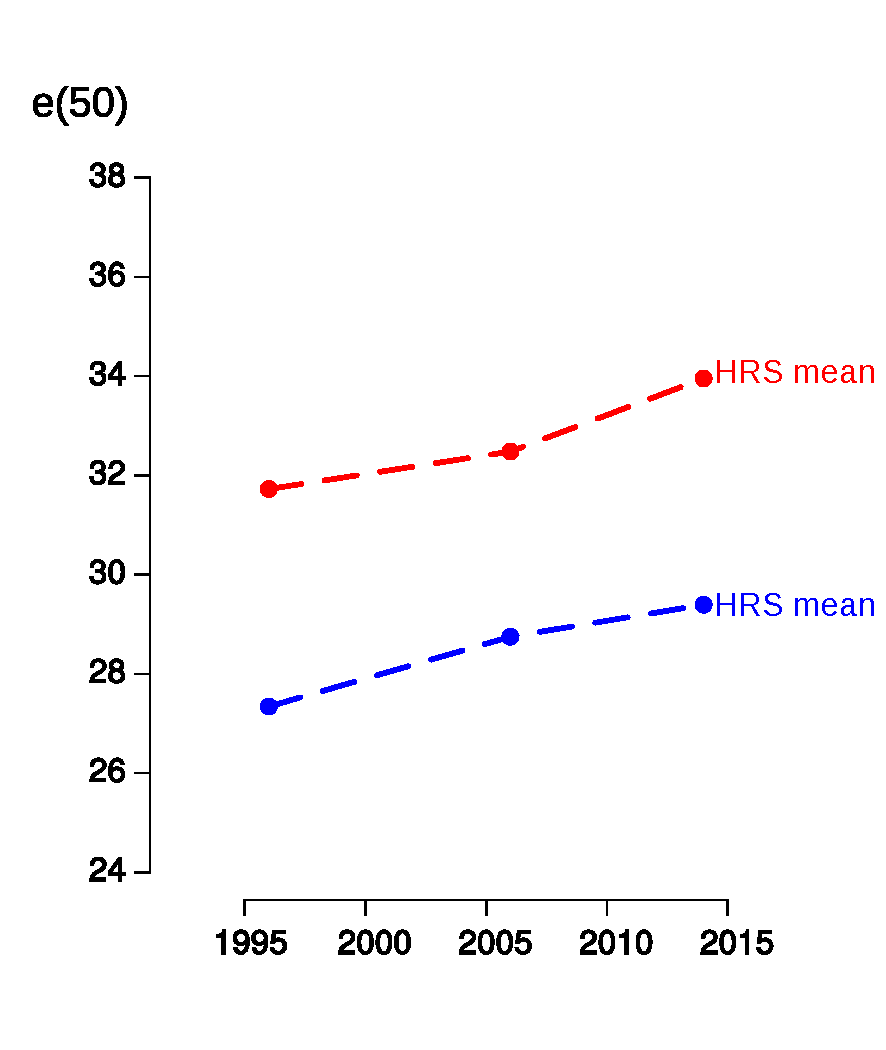
\includegraphics[height=\textheight, keepaspectratio]{Figures/e50_3.pdf}}
%\only<5>{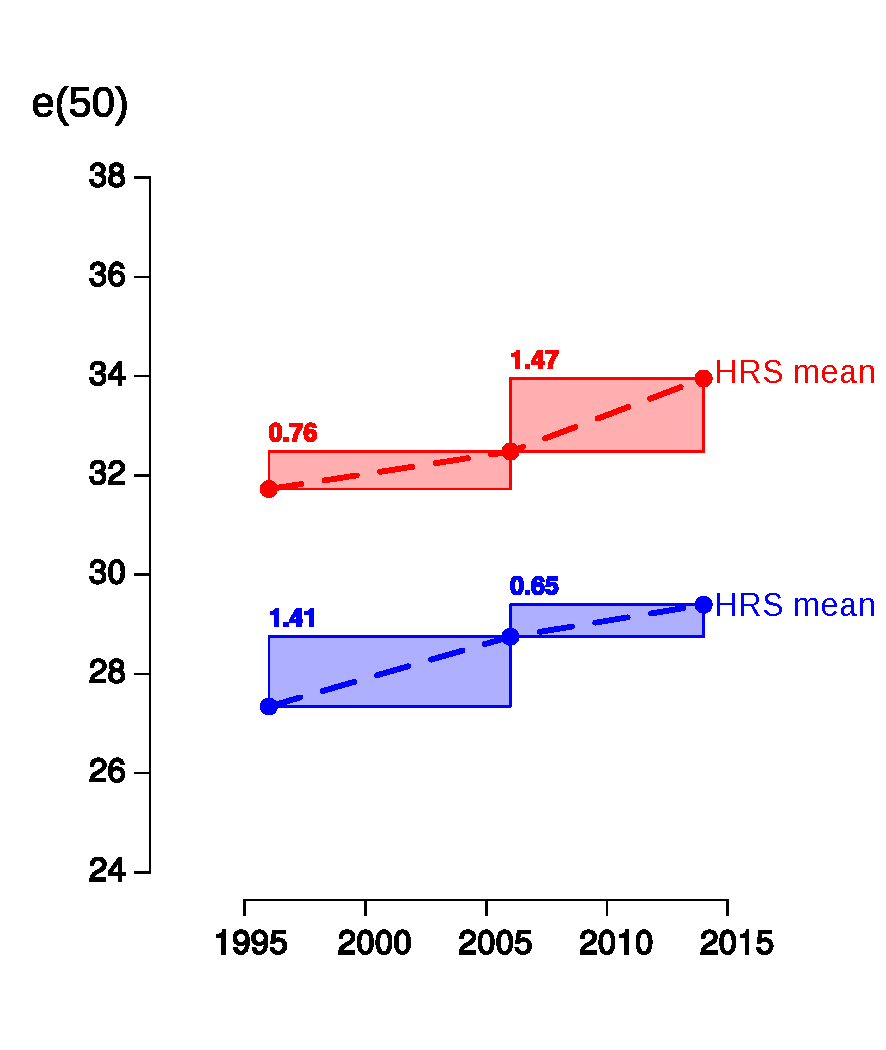
\includegraphics[height=\textheight, keepaspectratio]{Figures/e50_4.pdf}}
%\end{center}
%\end{overlayarea}
%\end{frame}
%

\begin{frame}[plain]
\Large\begin{center}
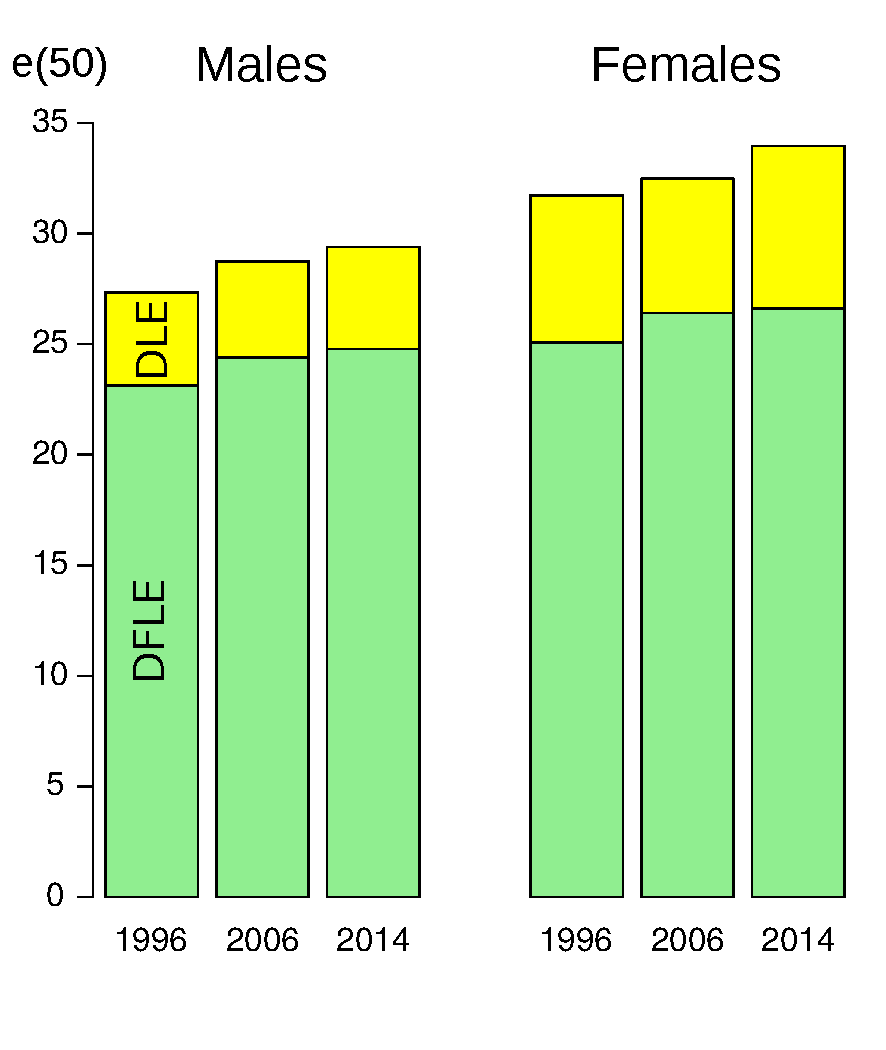
\includegraphics[height=\textheight, keepaspectratio]{Figures/lemf_ink.pdf}
\end{center}
\end{frame}

\begin{frame}[plain]
\Large
A word on decomposition
\vspace{2em}
\begin{itemize}[<+->]
\item If discrete, decompose wrt ``out'' probabilities.
\item all parameters in a single vector, $\textbf{p}$
\item wrap all programming steps to produce output $e(50)$ in a single function, $f(\textbf{p})$
\item I used \texttt{DemoDecomp} package
\end{itemize}
\end{frame}

\begin{frame}[plain]
\Large
\begin{center}
Males 1996-2006
\vspace{1em}

 \begin{tabular}{rrr|r}
      % latex table generated in R 3.5.1 by xtable 1.8-3 package
% Wed Sep 19 13:33:03 2018
 & DFLE & DLE & LE \\ 
  \midrule
Disablement & \cellcolor[HTML]{CEEBC8}{\color[HTML]{000000}0.31} & \cellcolor[HTML]{EEE4EF}{\color[HTML]{000000}-0.18} & \cellcolor[HTML]{E7F3E4}{\color[HTML]{000000}0.13} \\ 
  DF Mortality & \cellcolor[HTML]{358C46}{\color[HTML]{FFFFFF}1.00} & \cellcolor[HTML]{E7F3E4}{\color[HTML]{000000}0.12} & \cellcolor[HTML]{1D7938}{\color[HTML]{FFFFFF}1.12} \\ 
  Recovery & \cellcolor[HTML]{F4F0F4}{\color[HTML]{000000}-0.04} & \cellcolor[HTML]{F1F5F0}{\color[HTML]{000000}0.03} & \cellcolor[HTML]{F4F0F4}{\color[HTML]{000000}-0.01} \\ 
  Dis. Mortality & \cellcolor[HTML]{E7F3E4}{\color[HTML]{000000}0.12} & \cellcolor[HTML]{F1F5F0}{\color[HTML]{000000}0.03} & \cellcolor[HTML]{E7F3E4}{\color[HTML]{000000}0.14} \\ 
   \midrule
Age 50 Disab. & \cellcolor[HTML]{F4F0F4}{\color[HTML]{000000}-0.03} & \cellcolor[HTML]{F1F5F0}{\color[HTML]{000000}0.01} & \cellcolor[HTML]{F4F0F4}{\color[HTML]{000000}-0.02} \\ 
  Age 50 Educ. & \cellcolor[HTML]{E7F3E4}{\color[HTML]{000000}0.13} & \cellcolor[HTML]{F4F0F4}{\color[HTML]{000000}-0.03} & \cellcolor[HTML]{F1F5F0}{\color[HTML]{000000}0.09} \\ 
   \midrule
Total & \cellcolor[HTML]{00441A}{\color[HTML]{FFFFFF}1.49} & \cellcolor[HTML]{F4F0F4}{\color[HTML]{000000}-0.03} & \cellcolor[HTML]{00441A}{\color[HTML]{FFFFFF}1.46} \\ 
  
     \end{tabular}
     \end{center}
\end{frame}
\begin{frame}[plain]
\Large
\begin{center}
Males 2006-2014
\vspace{1em}

      \begin{tabular}{rrr|r}
      % latex table generated in R 3.5.1 by xtable 1.8-3 package
% Wed Sep 19 13:33:04 2018
 & DFLE & DLE & LE \\ 
  \midrule
Disablement & \cellcolor[HTML]{E7F3E4}{\color[HTML]{000000}0.15} & \cellcolor[HTML]{F4F0F4}{\color[HTML]{000000}-0.09} & \cellcolor[HTML]{F1F5F0}{\color[HTML]{000000}0.06} \\ 
  DF Mortality & \cellcolor[HTML]{ABDDA5}{\color[HTML]{000000}0.52} & \cellcolor[HTML]{F1F5F0}{\color[HTML]{000000}0.06} & \cellcolor[HTML]{ABDDA5}{\color[HTML]{000000}0.58} \\ 
  Recovery & \cellcolor[HTML]{E9D8EA}{\color[HTML]{000000}-0.26} & \cellcolor[HTML]{E7F3E4}{\color[HTML]{000000}0.13} & \cellcolor[HTML]{EEE4EF}{\color[HTML]{000000}-0.13} \\ 
  Dis. Mortality & \cellcolor[HTML]{F1F5F0}{\color[HTML]{000000}0.09} & \cellcolor[HTML]{F1F5F0}{\color[HTML]{000000}0.03} & \cellcolor[HTML]{E7F3E4}{\color[HTML]{000000}0.12} \\ 
   \midrule
Age 50 Disab. & \cellcolor[HTML]{F4F0F4}{\color[HTML]{000000}-0.05} & \cellcolor[HTML]{F1F5F0}{\color[HTML]{000000}0.02} & \cellcolor[HTML]{F4F0F4}{\color[HTML]{000000}-0.04} \\ 
  Age 50 Educ. & \cellcolor[HTML]{F1F5F0}{\color[HTML]{000000}0.09} & \cellcolor[HTML]{F4F0F4}{\color[HTML]{000000}-0.02} & \cellcolor[HTML]{F1F5F0}{\color[HTML]{000000}0.07} \\ 
   \midrule
Total & \cellcolor[HTML]{ABDDA5}{\color[HTML]{000000}0.54} & \cellcolor[HTML]{E7F3E4}{\color[HTML]{000000}0.12} & \cellcolor[HTML]{94D090}{\color[HTML]{000000}0.67} \\ 
  
     \end{tabular}
     \end{center}
\end{frame}
  
  
\begin{frame}[plain]
\Large
\begin{center}
Females 1996-2006
\vspace{1em}

 \begin{tabular}{rrr|r}
      % latex table generated in R 3.5.1 by xtable 1.8-3 package
% Wed Sep 19 13:33:03 2018
 & DFLE & DLE & LE \\ 
  \midrule
Onset & \cellcolor[HTML]{ABDDA5}{\color[HTML]{000000}0.59} & \cellcolor[HTML]{DFCAE2}{\color[HTML]{000000}-0.34} & \cellcolor[HTML]{DDF1D7}{\color[HTML]{000000}0.26} \\ 
  DF Mortality & \cellcolor[HTML]{7AC07A}{\color[HTML]{000000}0.76} & \cellcolor[HTML]{F1F5F0}{\color[HTML]{000000}0.09} & \cellcolor[HTML]{5FB165}{\color[HTML]{FFFFFF}0.85} \\ 
  Recovery & \cellcolor[HTML]{F1F5F0}{\color[HTML]{000000}0.07} & \cellcolor[HTML]{F4F0F4}{\color[HTML]{000000}-0.01} & \cellcolor[HTML]{F1F5F0}{\color[HTML]{000000}0.06} \\ 
  Dis. Mortality & \cellcolor[HTML]{DFCAE2}{\color[HTML]{000000}-0.39} & \cellcolor[HTML]{F4F0F4}{\color[HTML]{000000}-0.08} & \cellcolor[HTML]{D2B9DA}{\color[HTML]{000000}-0.47} \\ 
   \midrule
Age 50 Disab. & \cellcolor[HTML]{EEE4EF}{\color[HTML]{000000}-0.14} & \cellcolor[HTML]{F1F5F0}{\color[HTML]{000000}0.05} & \cellcolor[HTML]{F4F0F4}{\color[HTML]{000000}-0.09} \\ 
  Age 50 Educ. & \cellcolor[HTML]{F1F5F0}{\color[HTML]{000000}0.09} & \cellcolor[HTML]{F4F0F4}{\color[HTML]{000000}-0.01} & \cellcolor[HTML]{F1F5F0}{\color[HTML]{000000}0.08} \\ 
   \midrule
Total & \cellcolor[HTML]{499E55}{\color[HTML]{FFFFFF}0.99} & \cellcolor[HTML]{E9D8EA}{\color[HTML]{000000}-0.30} & \cellcolor[HTML]{94D090}{\color[HTML]{000000}0.69} \\ 
  
     \end{tabular}
      \end{center}
\end{frame}
\begin{frame}[plain]
\Large
\begin{center}
Females 2006-2014

\vspace{1em}
      \begin{tabular}{rrr|r}
      % latex table generated in R 3.5.1 by xtable 1.8-3 package
% Wed Sep 19 13:33:03 2018
 & DFLE & DLE & LE \\ 
  \midrule
Onset & \cellcolor[HTML]{F4F0F4}{\color[HTML]{000000}-0.00} & \cellcolor[HTML]{F4F0F4}{\color[HTML]{000000}-0.01} & \cellcolor[HTML]{F4F0F4}{\color[HTML]{000000}-0.02} \\ 
  DF Mortality & \cellcolor[HTML]{12672E}{\color[HTML]{FFFFFF}1.21} & \cellcolor[HTML]{E7F3E4}{\color[HTML]{000000}0.15} & \cellcolor[HTML]{075524}{\color[HTML]{FFFFFF}1.36} \\ 
  Recovery & \cellcolor[HTML]{834692}{\color[HTML]{FFFFFF}-1.04} & \cellcolor[HTML]{94D090}{\color[HTML]{000000}0.62} & \cellcolor[HTML]{D2B9DA}{\color[HTML]{000000}-0.42} \\ 
  Dis. Mortality & \cellcolor[HTML]{CEEBC8}{\color[HTML]{000000}0.38} & \cellcolor[HTML]{F1F5F0}{\color[HTML]{000000}0.08} & \cellcolor[HTML]{BDE4B6}{\color[HTML]{000000}0.45} \\ 
   \midrule
Age 50 Disab. & \cellcolor[HTML]{E9D8EA}{\color[HTML]{000000}-0.29} & \cellcolor[HTML]{E7F3E4}{\color[HTML]{000000}0.10} & \cellcolor[HTML]{EEE4EF}{\color[HTML]{000000}-0.19} \\ 
  Age 50 Educ. & \cellcolor[HTML]{EEE4EF}{\color[HTML]{000000}-0.14} & \cellcolor[HTML]{F1F5F0}{\color[HTML]{000000}0.05} & \cellcolor[HTML]{F4F0F4}{\color[HTML]{000000}-0.09} \\ 
   \midrule
Total & \cellcolor[HTML]{E7F3E4}{\color[HTML]{000000}0.12} & \cellcolor[HTML]{499E55}{\color[HTML]{FFFFFF}0.98} & \cellcolor[HTML]{1D7938}{\color[HTML]{FFFFFF}1.10} \\ 
  
     \end{tabular}
     \end{center}
\end{frame}     
 
\begin{frame}[plain]
\Large
\begin{center}
Some thoughts
\begin{itemize}[<+->]
\item Why decompose?
\item Additivity
\item Multidimensional output: tables, bars, other, or none?
\end{itemize}
\end{center}
\end{frame}
%%%%%%%%%%%%%%%%%%%%%%%%%%%%%%%%%%
%%	End of the document			%%
%%%%%%%%%%%%%%%%%%%%%%%%%%%%%%%%%%
\end{document}






